\section{Conveyor movement and falling}
\label{sec:transfer}
\begin{figure}[H]\centering
\begin{minipage}{0.49\linewidth}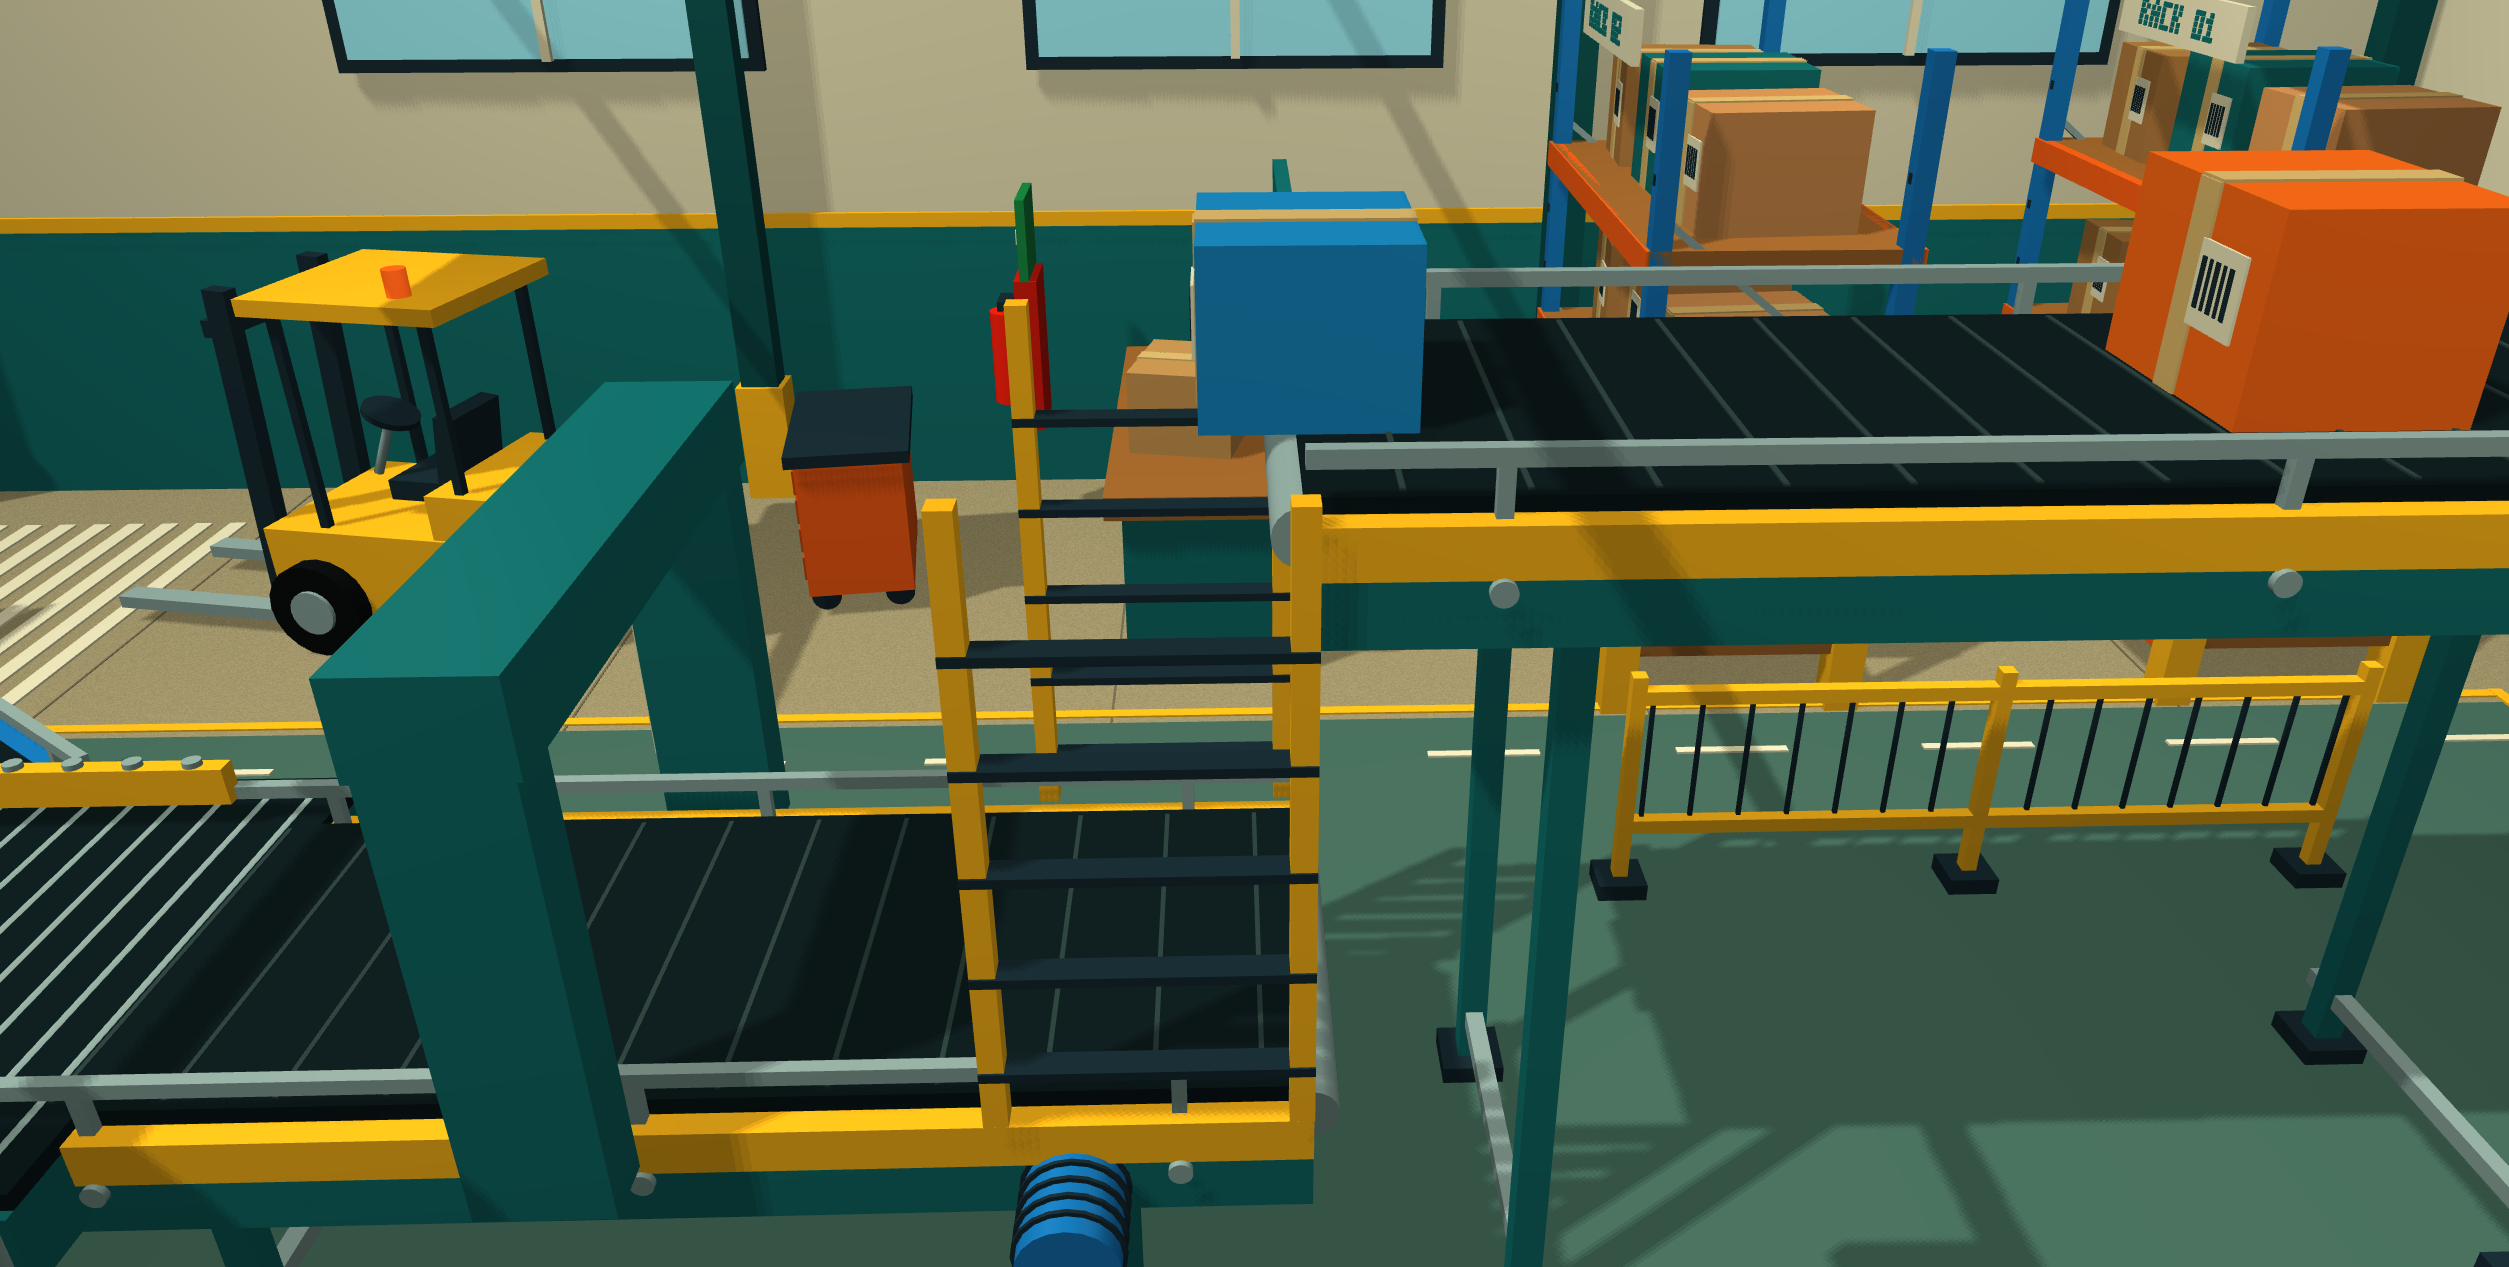
\includegraphics[width=\linewidth]{assets/transfer_before_crop.png}\par\small\textbf{A. 4.10 s:} first blue box approaches the upper belt edge.\end{minipage}\hfill
\begin{minipage}{0.49\linewidth}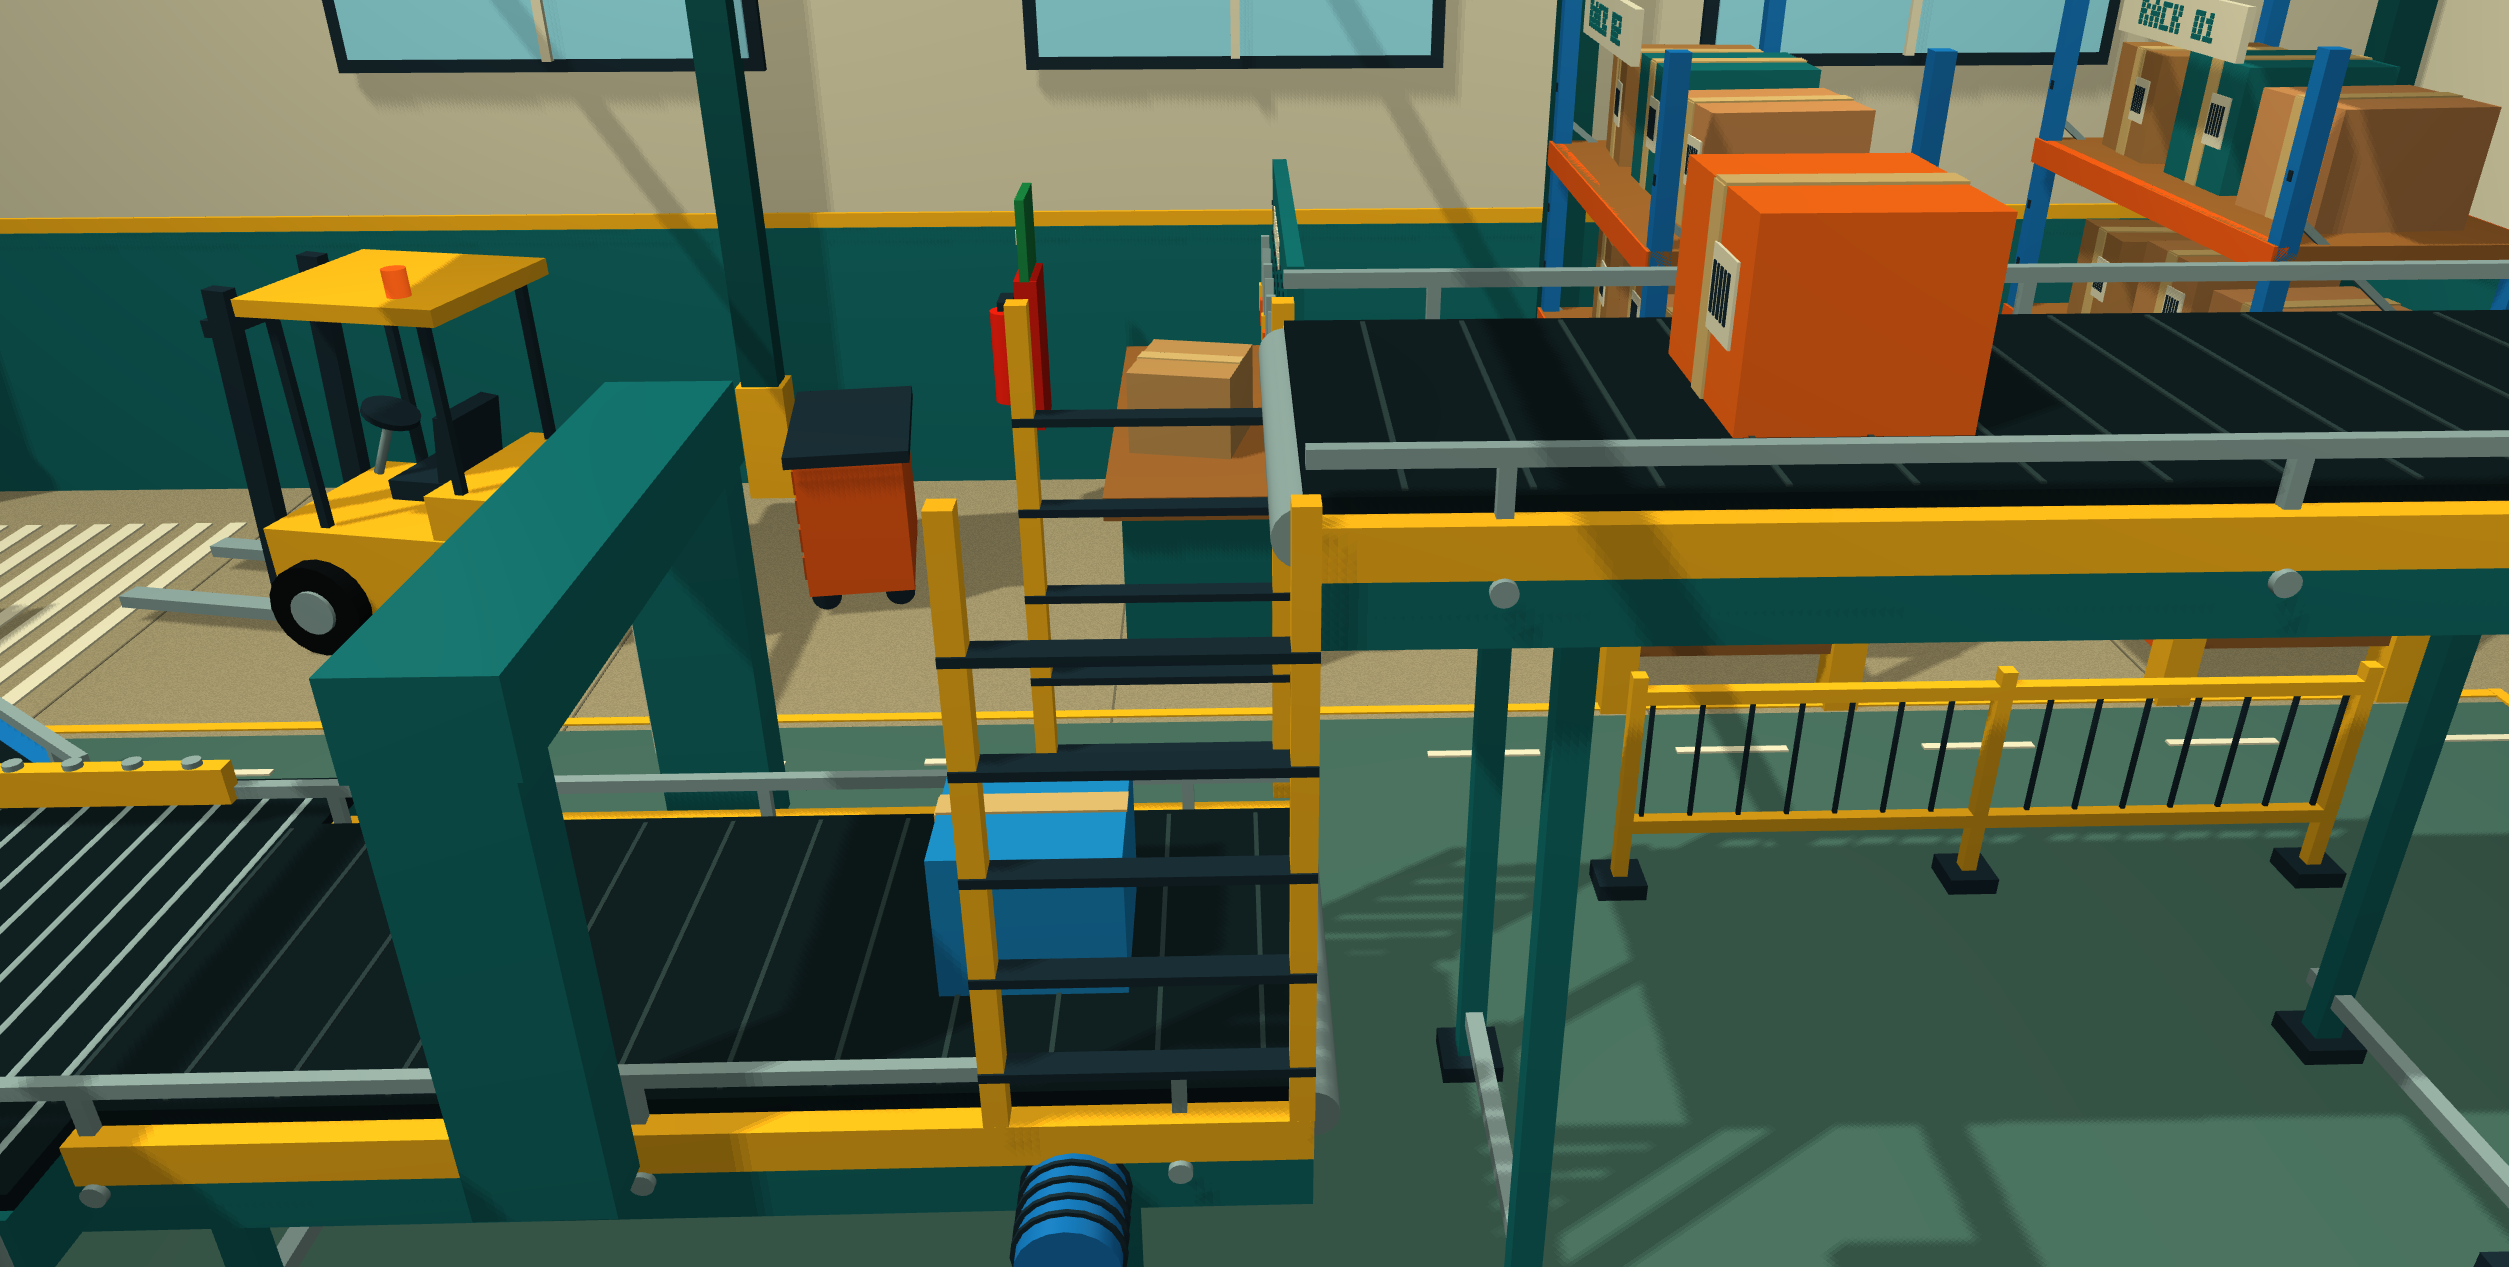
\includegraphics[width=\linewidth]{assets/transfer_landed_crop.png}\par\small\textbf{B. 5.30 s:} it has landed on the lower belt.\end{minipage}
\caption{Before and after the transfer, using the same camera and image crop.}
\end{figure}
\begin{shot}[0.80\linewidth]{assets/transfer_fall_crop.png}{At 4.75 s the box is falling and tilted. This close view shows the gap between the two conveyor levels.}
\callout{0.44,0.63}{0.20,0.90}{Falling box}
\callout{0.64,0.67}{0.85,0.94}{Upper belt}
\callout{0.22,0.15}{0.19,0.08}{Lower belt}
\end{shot}
\subsection{Motion model}
On a conveyor, the position update is $z'=z+v\Delta t$, where $v$ is speed and $\Delta t$ is elapsed time. The default speed is 1.55 units/s; keyboard input changes it by 0.20 within 0.65--3.00 units/s.

During a fall, the code first updates vertical velocity, then height:
\begin{equation}
v_y'=v_y-9.81\Delta t,\qquad y'=y+v_y'\Delta t.
\end{equation}
The parcel also moves forward by $0.62\Delta t$. On landing, the center height is constrained to $1.45+0.10+h/2$, where $h$ is box height. Tilt is $16^\circ\sin(\pi\min(1,t/0.72))$; it returns to zero on landing.

\textbf{Spacing:} required center gap is $(l_i+l_a)/2+0.40$. A box waits when the receiver is occupied. Updates use steps of at most $1/120$ s and cap a frame's accepted time at 0.25 s. End rollers use $\theta'= (\theta+190v\Delta t)\bmod360$; repeating strips suggest belt movement. These roller rates are visual choices.
\source{\code{FactorySimulation.cpp}: \code{update()}, \code{advanceOnBelt()}, falling case; \code{FactoryScene.cpp}: conveyor/box drawing.}
